Dans la lignée de pensée de \citet{milia2023}, nous considérons un texte comme point d'entrée pour étudier les tendances de la circulation des idées à l'aide des caractéristiques structurelles spécifiques (en l'occurrence, les termes linguistiques désignant les concepts médicaux). C'est par l'entremise de ce constat que découle la question de savoir \textit{s'il est possible de mesurer l'impact de Charcot sur l'histoire des neurosciences à travers les termes scientifiques qu'il a employés et qui ont été repris par son réseau scientifique}. En l'occurrence, nous avançons l'hypothèse que certains termes médicaux dont Charcot a été l'inventeur ou le transmetteur ont été repris de manière significative dans les écrits de son réseau. Ces termes se déclinent sous forme des unigrammes (mots uniques), mais aussi des expressions à mots multiples (angl. \textit{multi-word expressions}), plus précisément des collocations, \og{}associations conventionnelles de mots, arbitraires et récurrentes, dont les éléments ne sont pas nécessairement contigus et dont la signification est largement transparente\fg{} \citep[p. 96]{nerima2006}. La complexité syntaxique de ces termes, qui constituent le champ notionnel médical et potentiellement des savoirs en circulation, peut être résumée ainsi :
\begin{table}[h]
	\centering
	\begin{tabular}{l|l}
		\multicolumn{1}{c|}{Partie(s) du discours} & \multicolumn{1}{c}{Exemple} \\
		\hline
		\textsc{nom} & \textit{hystérie}\\
		\textsc{nom + adjectif} & \textit{ataxie locomotrice}\\
		\textsc{nom + adjectif + adjectif} & \textit{sclérose latérale amyotrophique}\\
		\textsc{nom + préposition + nom + adjectif} & \textit{état de mal hystéro-épileptique}
	\end{tabular}
	\caption{Exemples des concepts scientifiques avec leurs parties du discours.}
\end{table}

À ce titre, nous nous tâchons à mesurer informatiquement l'impact des travaux de Charcot sur son réseau scientifique. Cette mesure se fonde sur l'analyse des concepts-clés en matière de son discours scientifique, et plus particulièrement sur l'opérationnalisation du terme \og{}influence\fg{}, définie ici comme une intertextualité uni-directionnelle, allant des écrits de Charcot (ci-après corpus \og{}Charcot\fg{}) vers ceux de son réseau scientifique (ci-après corpus \og{}Autres\fg{}). Il s'agit donc \textit{in fine} d'aborder computationnellement la question des circulations, non pas des artefacts matériels comme les manuscrits \citep{gabay2021katabase} et les images \citep{joyeux2019visual}, mais des phénomènes textuels complexes \citep{manjavacas} ayant une dimension théorique forte. Notre approche a été formalisée sur la figure \ref{fig:formalisation} : à partir des documents au format \textsc{PDF}, une océrisation puis une structuration au format \textsc{XML} ont été réalisées, ces étapes ayant été prises en charge par la \textsc{BSU}. Nous avons exploité ces fichiers en appliquant plusieurs méthodes d’extraction de termes médicaux sur les corpus Charcot et Autres. Les termes extraits ont ensuite été comparés à ceux de notre liste de référence (voir section \ref{sect:methodo_stat}), avec une évaluation qualitative fondée sur l'analyse de leur contexte d'utilisation.

\begin{figure}[!ht]
	\centering
	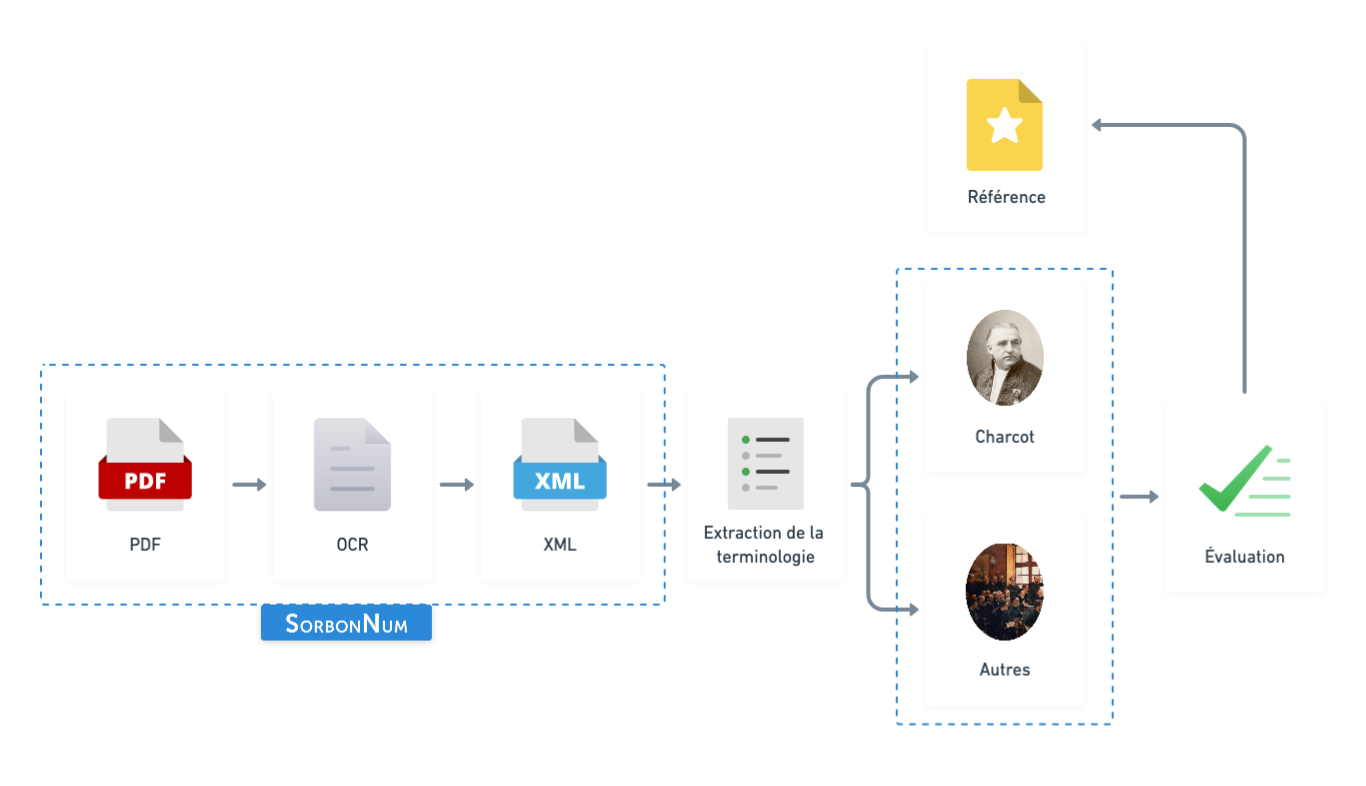
\includegraphics[width=1\textwidth]{img/formalisation_approche.png}
	\caption{Formalisation de l'approche pour pister la circulation des termes médicaux.}
	\label{fig:formalisation}
\end{figure}
